\documentclass{standalone}
\usepackage{tikz}
\usetikzlibrary{patterns, positioning}


\begin{document}
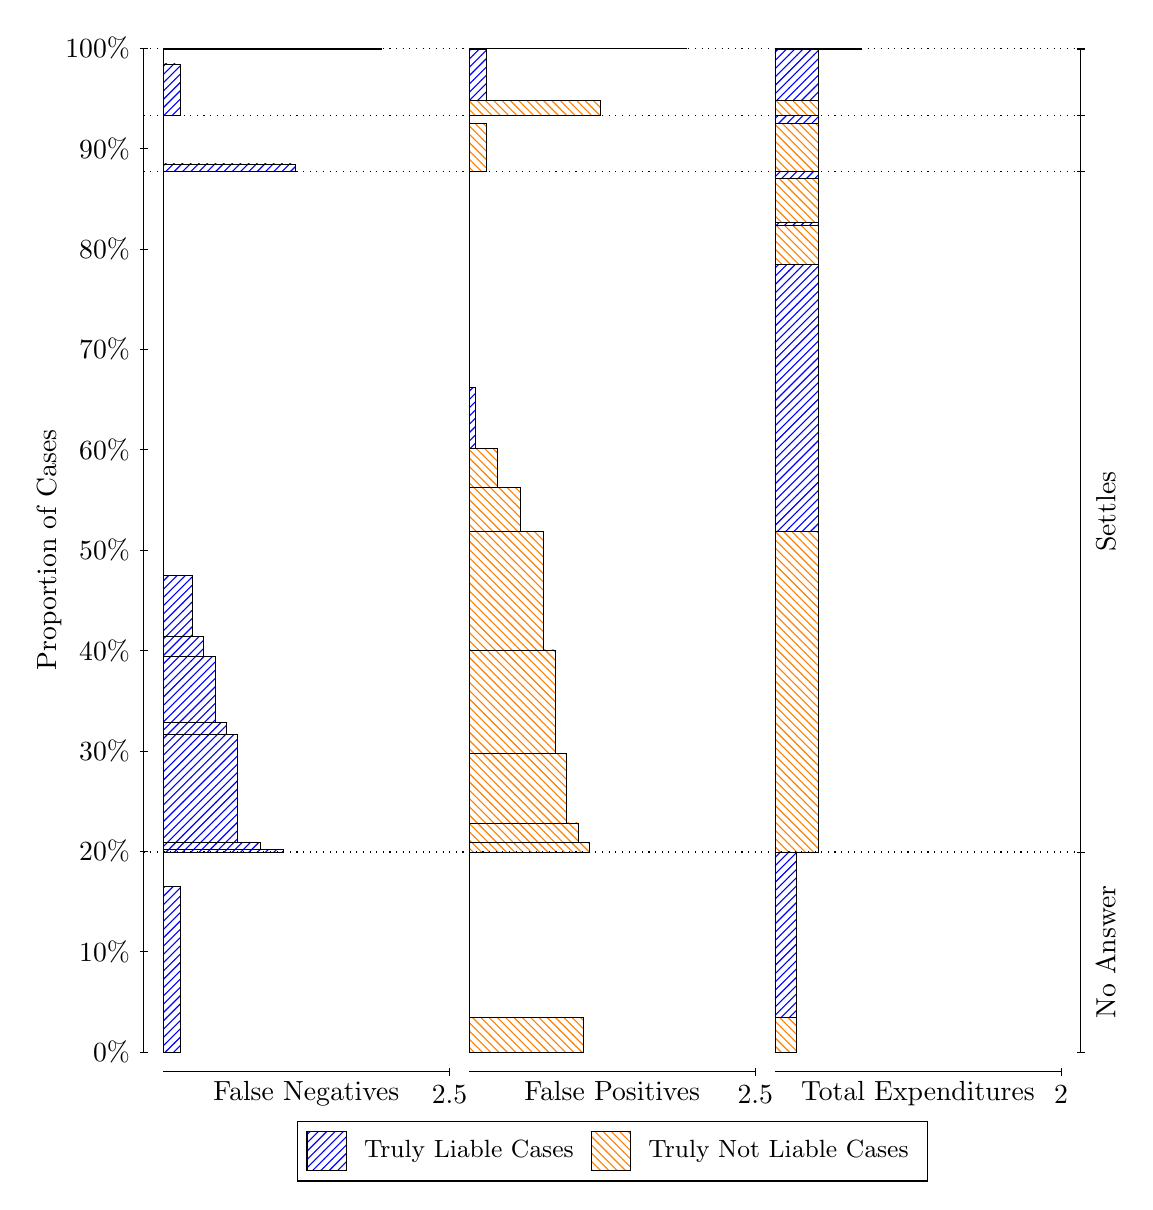
\begin{tikzpicture}
\draw[black, very thin] (1.5,1.75) -- (1.5,14.5);
\node[rotate=90, text=black, anchor=center] at (0.3, 8.125) {Proportion of Cases};
\draw[black, very thin] (1.45,1.75) -- (1.55,1.75);
\node[text=black, anchor=east] at (1.45, 1.75) {0\%};
\draw[black, very thin] (1.45,3.025) -- (1.55,3.025);
\node[text=black, anchor=east] at (1.45, 3.025) {10\%};
\draw[black, very thin] (1.45,4.3) -- (1.55,4.3);
\node[text=black, anchor=east] at (1.45, 4.3) {20\%};
\draw[black, very thin] (1.45,5.575) -- (1.55,5.575);
\node[text=black, anchor=east] at (1.45, 5.575) {30\%};
\draw[black, very thin] (1.45,6.85) -- (1.55,6.85);
\node[text=black, anchor=east] at (1.45, 6.85) {40\%};
\draw[black, very thin] (1.45,8.125) -- (1.55,8.125);
\node[text=black, anchor=east] at (1.45, 8.125) {50\%};
\draw[black, very thin] (1.45,9.4) -- (1.55,9.4);
\node[text=black, anchor=east] at (1.45, 9.4) {60\%};
\draw[black, very thin] (1.45,10.675) -- (1.55,10.675);
\node[text=black, anchor=east] at (1.45, 10.675) {70\%};
\draw[black, very thin] (1.45,11.95) -- (1.55,11.95);
\node[text=black, anchor=east] at (1.45, 11.95) {80\%};
\draw[black, very thin] (1.45,13.225) -- (1.55,13.225);
\node[text=black, anchor=east] at (1.45, 13.225) {90\%};
\draw[black, very thin] (1.45,14.5) -- (1.55,14.5);
\node[text=black, anchor=east] at (1.45, 14.5) {100\%};

\draw[black, very thin] (13.4,1.75) -- (13.4,14.5);
\draw[black, very thin] (13.35,1.75) -- (13.45,1.75);
\node[anchor=west] at (13.35, 1.75) {};
\draw[black, very thin] (13.35,4.2901) -- (13.45,4.2901);
\node[anchor=west] at (13.35, 4.2901) {};
\draw[black, very thin] (13.35,12.934) -- (13.45,12.934);
\node[anchor=west] at (13.35, 12.934) {};
\draw[black, very thin] (13.35,13.64) -- (13.45,13.64);
\node[anchor=west] at (13.35, 13.64) {};
\draw[black, very thin] (13.35,14.49) -- (13.45,14.49);
\node[anchor=west] at (13.35, 14.49) {};
\draw[black, very thin] (13.35,14.495) -- (13.45,14.495);
\node[anchor=west] at (13.35, 14.495) {};
\draw[black, very thin] (13.35,14.5) -- (13.45,14.5);
\node[anchor=west] at (13.35, 14.5) {};

\draw[black, very thin, pattern color=blue, pattern=north east lines] (1.75,1.75) rectangle (1.968,3.8529);
\draw[black, very thin, pattern color=orange, pattern=north west lines] (1.75,3.8529) rectangle (1.75,4.2901);
\draw[black, very thin, pattern color=blue, pattern=north east lines] (1.75,4.2901) rectangle (3.276,4.3236);
\draw[black, very thin, pattern color=blue, pattern=north east lines] (1.75,4.3236) rectangle (2.9853,4.4106);
\draw[black, very thin, pattern color=blue, pattern=north east lines] (1.75,4.4106) rectangle (2.6947,5.7786);
\draw[black, very thin, pattern color=blue, pattern=north east lines] (1.75,5.7786) rectangle (2.5493,5.9354);
\draw[black, very thin, pattern color=blue, pattern=north east lines] (1.75,5.9354) rectangle (2.404,6.7696);
\draw[black, very thin, pattern color=blue, pattern=north east lines] (1.75,6.7696) rectangle (2.2587,7.0305);
\draw[black, very thin, pattern color=blue, pattern=north east lines] (1.75,7.0305) rectangle (2.1133,7.8058);
\draw[black, very thin, pattern color=orange, pattern=north west lines] (1.75,7.8058) rectangle (1.75,12.934);
\draw[black, very thin, pattern color=blue, pattern=north east lines] (1.75,12.934) rectangle (3.4213,13.028);
\draw[black, very thin, pattern color=orange, pattern=north west lines] (1.75,13.028) rectangle (1.75,13.64);
\draw[black, very thin, pattern color=blue, pattern=north east lines] (1.75,13.64) rectangle (1.968,14.298);
\draw[black, very thin, pattern color=orange, pattern=north west lines] (1.75,14.298) rectangle (1.75,14.49);
\draw[black, very thin, pattern color=blue, pattern=north east lines] (1.75,14.49) rectangle (4.5113,14.492);
\draw[black, very thin, pattern color=orange, pattern=north west lines] (1.75,14.492) rectangle (1.75,14.495);
\draw[black, very thin, pattern color=orange, pattern=north west lines] (1.75,14.495) rectangle (1.75,14.497);
\draw[black, very thin, pattern color=blue, pattern=north east lines] (1.75,14.497) rectangle (1.75,14.5);
\draw[black, very thin, pattern color=orange, pattern=north west lines] (5.6333,1.75) rectangle (7.0867,2.1872);
\draw[black, very thin, pattern color=blue, pattern=north east lines] (5.6333,2.1872) rectangle (5.6333,4.2901);
\draw[black, very thin, pattern color=orange, pattern=north west lines] (5.6333,4.2901) rectangle (7.1593,4.4151);
\draw[black, very thin, pattern color=orange, pattern=north west lines] (5.6333,4.4151) rectangle (7.014,4.6595);
\draw[black, very thin, pattern color=orange, pattern=north west lines] (5.6333,4.6595) rectangle (6.8687,5.5429);
\draw[black, very thin, pattern color=orange, pattern=north west lines] (5.6333,5.5429) rectangle (6.7233,6.8573);
\draw[black, very thin, pattern color=orange, pattern=north west lines] (5.6333,6.8573) rectangle (6.578,8.3613);
\draw[black, very thin, pattern color=orange, pattern=north west lines] (5.6333,8.3613) rectangle (6.2873,8.9244);
\draw[black, very thin, pattern color=orange, pattern=north west lines] (5.6333,8.9244) rectangle (5.9967,9.4184);
\draw[black, very thin, pattern color=blue, pattern=north east lines] (5.6333,9.4184) rectangle (5.706,10.194);
\draw[black, very thin, pattern color=blue, pattern=north east lines] (5.6333,10.194) rectangle (5.6333,12.934);
\draw[black, very thin, pattern color=orange, pattern=north west lines] (5.6333,12.934) rectangle (5.8513,13.546);
\draw[black, very thin, pattern color=blue, pattern=north east lines] (5.6333,13.546) rectangle (5.6333,13.64);
\draw[black, very thin, pattern color=orange, pattern=north west lines] (5.6333,13.64) rectangle (7.3047,13.833);
\draw[black, very thin, pattern color=blue, pattern=north east lines] (5.6333,13.833) rectangle (5.8513,14.49);
\draw[black, very thin, pattern color=orange, pattern=north west lines] (5.6333,14.49) rectangle (5.6333,14.494);
\draw[black, very thin, pattern color=blue, pattern=north east lines] (5.6333,14.494) rectangle (5.6333,14.495);
\draw[black, very thin, pattern color=orange, pattern=north west lines] (5.6333,14.495) rectangle (8.3947,14.497);
\draw[black, very thin, pattern color=blue, pattern=north east lines] (5.6333,14.497) rectangle (6.9413,14.5);
\draw[black, very thin, pattern color=orange, pattern=north west lines] (9.5167,1.75) rectangle (9.7892,2.1872);
\draw[black, very thin, pattern color=blue, pattern=north east lines] (9.5167,2.1872) rectangle (9.7892,4.2901);
\draw[black, very thin, pattern color=orange, pattern=north west lines] (9.5167,4.2901) rectangle (10.062,8.3613);
\draw[black, very thin, pattern color=blue, pattern=north east lines] (9.5167,8.3613) rectangle (10.062,11.756);
\draw[black, very thin, pattern color=orange, pattern=north west lines] (9.5167,11.756) rectangle (10.062,12.251);
\draw[black, very thin, pattern color=blue, pattern=north east lines] (9.5167,12.251) rectangle (10.062,12.284);
\draw[black, very thin, pattern color=orange, pattern=north west lines] (9.5167,12.284) rectangle (10.062,12.847);
\draw[black, very thin, pattern color=blue, pattern=north east lines] (9.5167,12.847) rectangle (10.062,12.934);
\draw[black, very thin, pattern color=orange, pattern=north west lines] (9.5167,12.934) rectangle (10.062,13.546);
\draw[black, very thin, pattern color=blue, pattern=north east lines] (9.5167,13.546) rectangle (10.062,13.64);
\draw[black, very thin, pattern color=orange, pattern=north west lines] (9.5167,13.64) rectangle (10.062,13.833);
\draw[black, very thin, pattern color=blue, pattern=north east lines] (9.5167,13.833) rectangle (10.062,14.49);
\draw[black, very thin, pattern color=orange, pattern=north west lines] (9.5167,14.49) rectangle (10.607,14.494);
\draw[black, very thin, pattern color=blue, pattern=north east lines] (9.5167,14.494) rectangle (10.607,14.495);
\draw[black, very thin, pattern color=orange, pattern=north west lines] (9.5167,14.495) rectangle (10.607,14.497);
\draw[black, very thin, pattern color=blue, pattern=north east lines] (9.5167,14.497) rectangle (10.607,14.5);
\draw[black, dotted] (1.5,4.2901) -- (13.4,4.2901);
\draw[black, dotted] (1.5,12.934) -- (13.4,12.934);
\draw[black, dotted] (1.5,13.64) -- (13.4,13.64);
\draw[black, dotted] (1.5,14.49) -- (13.4,14.49);
\draw[black, dotted] (1.5,14.495) -- (13.4,14.495);
\draw[black, very thin] (1.75,1.5) -- (5.3833,1.5);
\node[text=black, anchor=north] at (3.5667, 1.5) {False Negatives};
\draw[black, very thin] (5.3833,1.45) -- (5.3833,1.55);
\node[text=black, anchor=north] at (5.3833, 1.45) {2.5};

\draw[black, very thin] (5.6333,1.5) -- (9.2667,1.5);
\node[text=black, anchor=north] at (7.45, 1.5) {False Positives};
\draw[black, very thin] (9.2667,1.45) -- (9.2667,1.55);
\node[text=black, anchor=north] at (9.2667, 1.45) {2.5};

\draw[black, very thin] (9.5167,1.5) -- (13.15,1.5);
\node[text=black, anchor=north] at (11.333, 1.5) {Total Expenditures};
\draw[black, very thin] (13.15,1.45) -- (13.15,1.55);
\node[text=black, anchor=north] at (13.15, 1.45) {2};

\node[text=black, centered, rotate=90] at (13.72, 3.0201) {No Answer};
\node[text=black, centered, rotate=90] at (13.72, 8.6121) {Settles};





\draw (7.449999999999999,1.5) node[draw=none] (baseCoordinate) {};
\begin{scope}[align=center]
        \matrix[scale=0.5, draw=black, below=0.5cm of baseCoordinate, nodes={draw}, column sep=0.1cm]{
            \node[rectangle, draw, minimum width=0.5cm, minimum height=0.5cm, pattern color=blue, pattern=north east lines] {}; &
            \node[draw=none, font=\small, text=black] (B) {Truly Liable Cases}; &
            \node[rectangle, draw, minimum width=0.5cm, minimum height=0.5cm, pattern color=orange, pattern=north west lines] {}; &
            \node[draw=none, font=\small, text=black] (B) {Truly Not Liable Cases}; \\
            };
\end{scope}

\end{tikzpicture}
\end{document}